%\chapter{\textit{RESTU'S AN ENGINE FOR SYNTHETIC THESPIAN UNITS} (RESTU)}
%\label{chap:RESTU}

\section{\textit{RESTU's an Engine for Synthetic Thespian Units} (RESTU)}
\label{sec:RESTU}

Pengembangan \textit{engine} ECA yang diberi nama \textit{RESTU's an Engine for Synthetic Thespian Units} (RESTU) ini berangkat dari konsep yang terdapat pada \textit{conversational agent}, yaitu gagasan akan mampunya komputer melakukan perbincangan dengan manusia dalam bahasa alami manusia. \textit{Conversational agent}, yang sebelumnya hanya mampu menerima masukan dan memberi keluaran dalam bentuk teks atau suara saja, kemudian berevolusi menjadi \textit{conversational agent} yang memiliki wujud, misalnya berupa karakter manusia dalam bentuk 3-dimensi (3D), yang dikenal sebagai \textit{embodied conversational agent} (ECA) atau \textit{embodied conversational interface agent}. Wujud yang dimiliki oleh agen memungkinkan lebih banyak cara yang dapat digunakan dalam komunikasi antara manusia dan komputer, misalnya arah tatapan mata, gerakan badan, dan mimik muka. Dengan kata lain, agen memiliki kemampuan untuk melakukan komunikasi non-verbal dengan pengguna, seperti yang dilakukan dalam komunikasi tatap muka antar manusia, sehingga berpotensi menciptakan komunikasi yang lebih alami dan pengalaman interaksi yang lebih kaya bagi pengguna.

Fitur dasar dari ECA yang dibangun dengan \textit{engine} ini adalah mampu melakukan perbincangan dengan penggunanya dalam Bahasa Indonesia. Fitur dasar produk ECA yang lain akan sangat bergantung pada peran agen virtual. Sebagai contoh, apabila produk ECA ditujukan untuk berperan sebagai asisten, agen virtual akan mampu memahami permintaan penggunanya dan berusaha mewujudkannya. Apabila produk ECA ditujukan untuk berperan sebagai pemandu museum, agen virtual akan mampu memahami pertanyaan pengguna dan berusaha untuk menjawab serta menjelaskannya. Meskipun demikian, perlu diingat bahwa tindakan-tindakan tersebut sangat bergantung pada pengetahuan yang dimiliki oleh agen virtual. Sebagai contoh, agen virtual yang berperan sebagai pemandu museum hanya dapat menjawab pertanyaan-pertanyaan terkait museum. Fitur yang lain adalah agen virtual diwujudkan dalam tampilan 3D yang dilengkapi dengan kemampuan menggerakkan anggota badannya. Selain dapat menggerakkan bibir saat berbicara, agen virtual dapat menengokkan kepalanya untuk memandang lawan bicaranya. Agen juga dapat menunjukkan pose tertentu untuk mencapai tujuannya, misalnya menunjukkan suatu gambar ke pengguna, atau sekedar untuk membangun suasana percakapan yang tidak kaku.

\begin{figure}[ht!]
\vskip 1em
\centering
 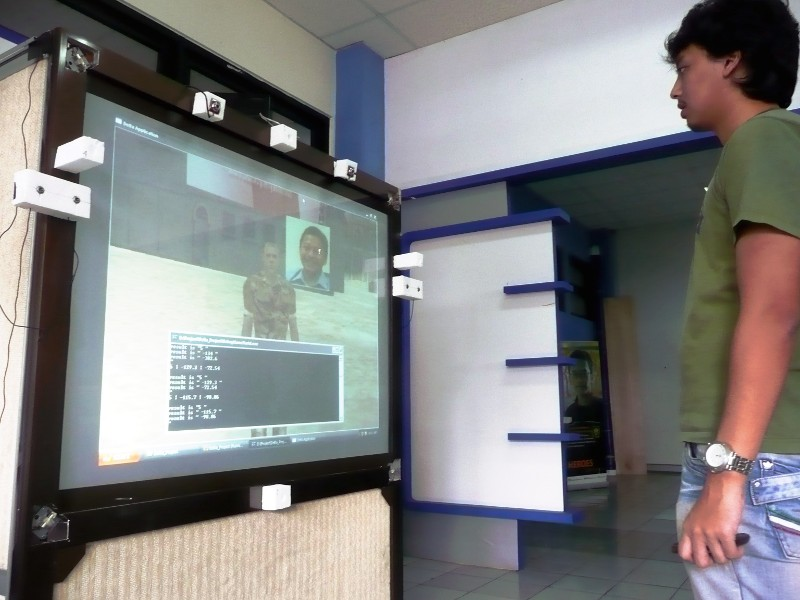
\includegraphics[width=0.9\textwidth,keepaspectratio=true]{images/prototipe_lskk.jpg}
 \caption[Interaksi pengguna dengan prototipe pemandu virtual LSKK yang dibangun dengan RESTU]{Interaksi pengguna dengan prototipe pemandu virtual LSKK yang dibangun dengan RESTU.}
 \label{fig:prototipe_lskk}
\vskip .5em
\end{figure}

Secara umum, RESTU disusun oleh teknologi pemrosesan bahasa alami, pemrosesan suara, pemrosesan citra, grafis 3D, dan kecerdasan artifisial. Teknologi pemrosesan bahasa alami, mencakup teknologi pengenalan suara dan sintesis suara. Teknologi pemrosesan suara digunakan dalam fungsi penentuan lokasi pengguna berdasarkan suara dan teknologi pemrosesan citra digunakan dalam fungsi pengenalan wajah untuk menentukan lokasi pengguna berdasarkan citra. Teknologi grafis digunakan untuk mewujudkan karakter virtual, perilakunya, dan lingkungannya. Sedangkan, teknologi kecerdasan artifisial dimanfaatkan untuk menyusun respons terhadap masukan dari pengguna yang diterima oleh agen berdasarkan pengetahuan yang dimilikinya.

Fungsi-fungsi yang menyusun RESTU tersebut dapat dikelompokkan menjadi dua bagian, yaitu bagian kognitif dan bagian interaksi. Fungsi kecerdasan artifisial menyusun bagian kognitif. Sedangkan, bagian interaksi tersusun dari fungsi pengenalan suara, sintesis suara, penentuan lokasi pengguna baik menggunakan suara mau pun citra, dan antarmuka grafis. Dengan mengikuti pengelompokan tersebut, di sisi implementasi RESTU dibangun dengan menggunakan dua kelompok \textit{server}, yaitu \textit{Artificial Intelligence (AI) Engine Server} dan \textit{User Interface (UI) Engine Server}. UI Engine Server dapat dibagi menjadi \textit{Camera Engine Server}, \textit{Speech Engine Server}, dan \textit{Graphical User Interface (GUI) Engine Server}. Diagram aliran data antar \textit{server}, atau modul yang ada di dalamnya, ditunjukkan oleh \autoref{fig:RESTU_arch}.

\begin{figure}[ht!]
\vskip 1em
\centering
 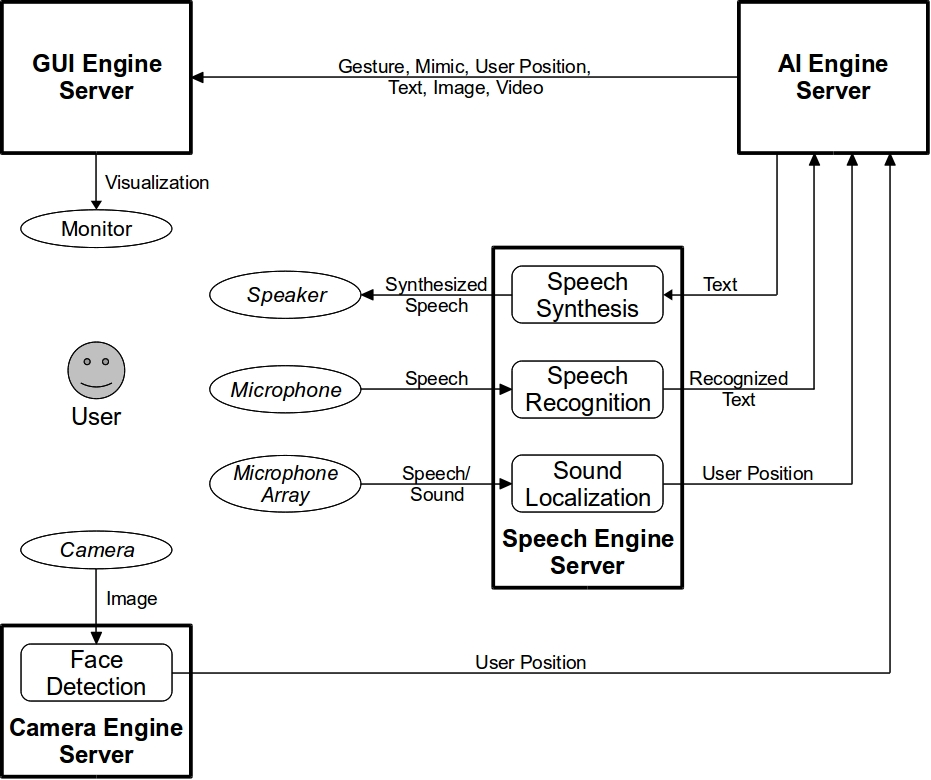
\includegraphics[width=.95\textwidth,keepaspectratio=true]{images/RESTU_arch.jpg}
 \caption[Diagram aliran data RESTU]{Diagram aliran data RESTU.}
 \label{fig:RESTU_arch}
\vskip .5em
\end{figure}
